\subsection{Dashboard - Tasa de crecimiento poblacional vs Consumo de energ�a a�o tras a�o}

\textsc{\begin{figure}[H]
	\centering
	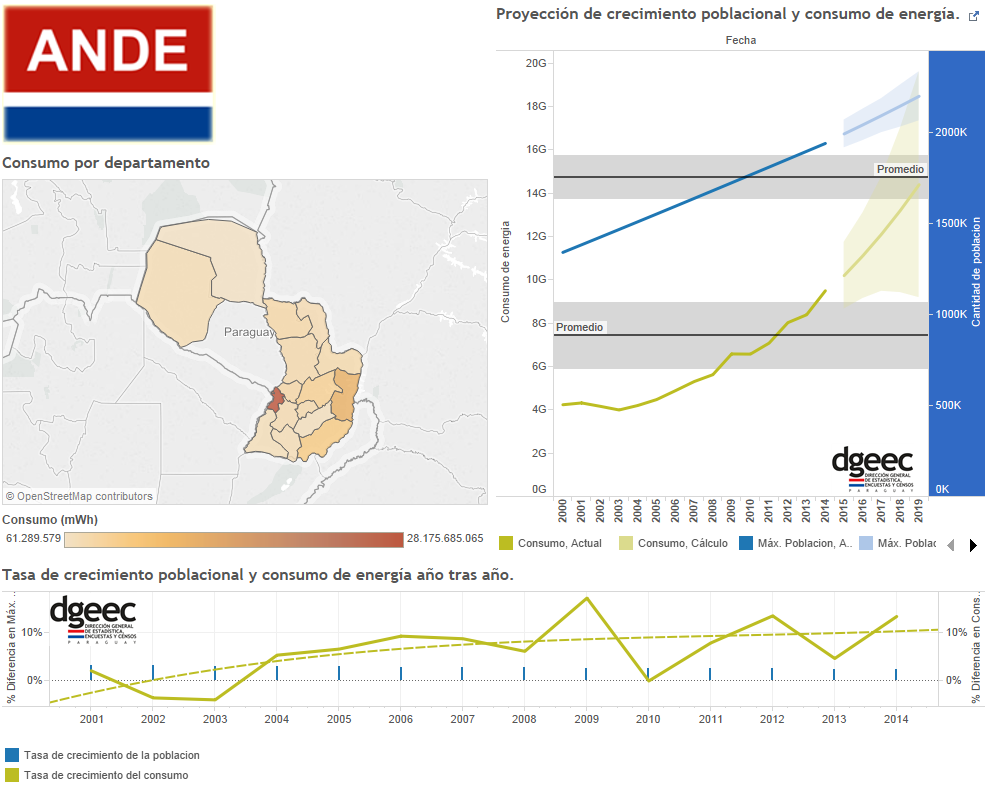
\includegraphics[width=\linewidth]{figuras/TasaDeCrecimientoPoblacionalYConsumoDeEnergiaAnoTrasAno}
	\caption{Dashboard - Tasa de crecimiento poblacional vs consumo de energ�a a�o tras a�o}
	\label{fig:TasaDeCrecimientoPoblacionalYConsumoDeEnergiaAnoTrasAno}
\end{figure}}

En el mapa, donde el color m�s oscuro representa al departamento que consume m�s energ�a el�ctrica y el color m�s claro, al que consume menos, vemos que los departamentos central, Alto Paran� son los que m�s demandan energ�a. Este tipo de gr�fico es muy �til cuando la informaci�n se quiere analizar de forma macro y georeferenciada. Al ubicar el mouse sobre cualquier departamento, se muestra un pop up indicando el valor de consumo del departamento seleccionado. Al dar clic sobre un departamento los dem�s gr�ficos tambi�n se actualizar�n en base a la selecci�n.

\textsc{\begin{figure}[H]
	\centering
	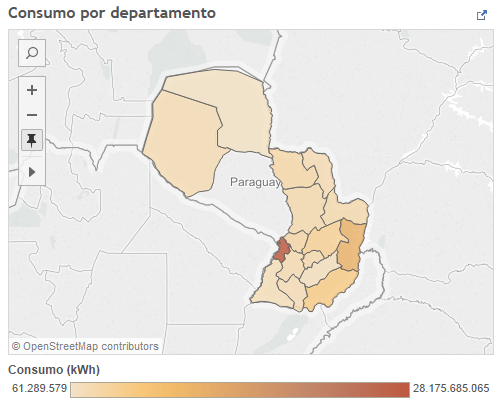
\includegraphics[width=\linewidth]{figuras/TasaDeCrecimientoPoblacionalYConsumoDeEnergiaAnoTrasAnoMapa}
	\caption{Consumo por departamento}
	\label{fig:TasaDeCrecimientoPoblacionalYConsumoDeEnergiaAnoTrasAnoMapa}
\end{figure}}

 En el segundo gr�fico, titulado ?Proyecci�n de crecimiento poblacional y consumo de energ�a?,  vemos el crecimiento de la poblaci�n (n�meros) y el crecimiento del consumo de energ�a el�ctrica expresado en GWh. Al seleccionar un departamento en el mapa, se puede analizar esta informaci�n por cada uno de ellos.


\textsc{\begin{figure}[H]
	\centering
	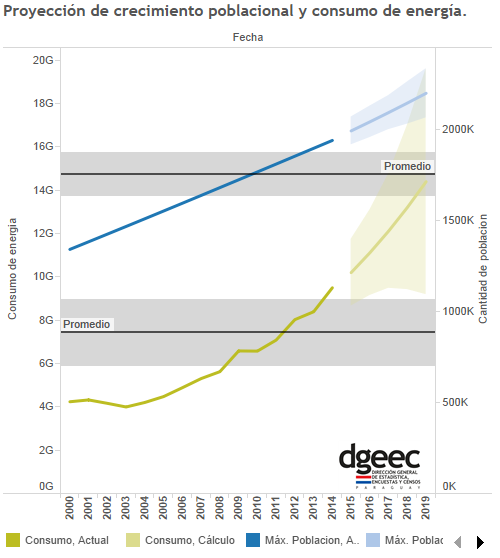
\includegraphics[width=\linewidth]{figuras/ProyeccionDeCrecimientoPoblacionalYConsumoDeEnergia}
	\caption{Proyecci�n de crecimiento poblacional y consumo ee energ�a}
	\label{fig:ProyeccionDeCrecimientoPoblacionalYConsumoDeEnergia}
\end{figure}}

En este gr�fico,  se muestra la misma informaci�n que el gr�fico anterior pero con diferente perspectiva, en este caso se calcula el porcentaje de crecimiento anual tanto de la poblaci�n, as� como del consumo.


\textsc{\begin{figure}[H]
	\centering
	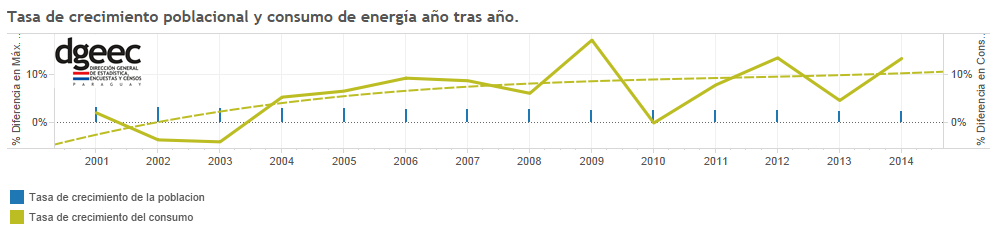
\includegraphics[width=\linewidth]{figuras/ProyeccionDeClientesYConsumosParaLosProximos5Anos2}
	\caption{Tasa de crecimiento poblacional y consumo ee energ�a a�os tras a�os}
	\label{fig:ProyeccionDeClientesYConsumosParaLosProximos5Anos2}
\end{figure}}